%!TEX root =../thesis. Tex
%*******************************************************************************
%****************************** Second Chapter *********************************
%*******************************************************************************

\chapter{The LHC and CMS}

\section{The Large Hadron Collider}

The Large Hadron Collider (LHC) is one the largest and most powerful particle accelerator in the world. It came on operation on 10 September 2008 and it is the most recent addition from the European Organization for Nuclear Research (CERN). The LHC is a 27 kilometer ring composed of superconducting magnets with accelerating structures to boost the energy of the particles. \\

The LHC is designed to accelerate particles to high energies and generate collisions. There are several
experiments installed along the LHC ring. One of them is ATLAS, located on Point 1 between the two injection lines, which is a general purpose detector. At point 5 is another general purpose detector: the compact muon solenoid (CMS). A particle detector optimized for heavy ion physics, ALICE, is located at Point 2 and LHCb, a detector designed for B physics, is located at Point 7.\cite{cern1,cern2}
\\

Inside the accelerator, two high energy particles beams travel at
close to the speed of light before they collide. 
In order to make them collide, beams travel in opposite directions in separate beam pipes, 
two tubes kept at ultrahigh vacuum. 
By using of superconducting electromagnets that generates a powerful magnetic field, the beams are guided around the accelerator ring. 
The electromagnets are built from coils of special electric cable that operates in a superconducting state, efficiently conducting electricity without resistance or loss of energy. For that, it is required to have magnets to a temperature of $‑271.3$ C. 
To reach such temperatures, a system of liquid helium is connected to the accelerator.\cite{cern2}

\pagebreak

\begin{figure}[!htbp]
\centering
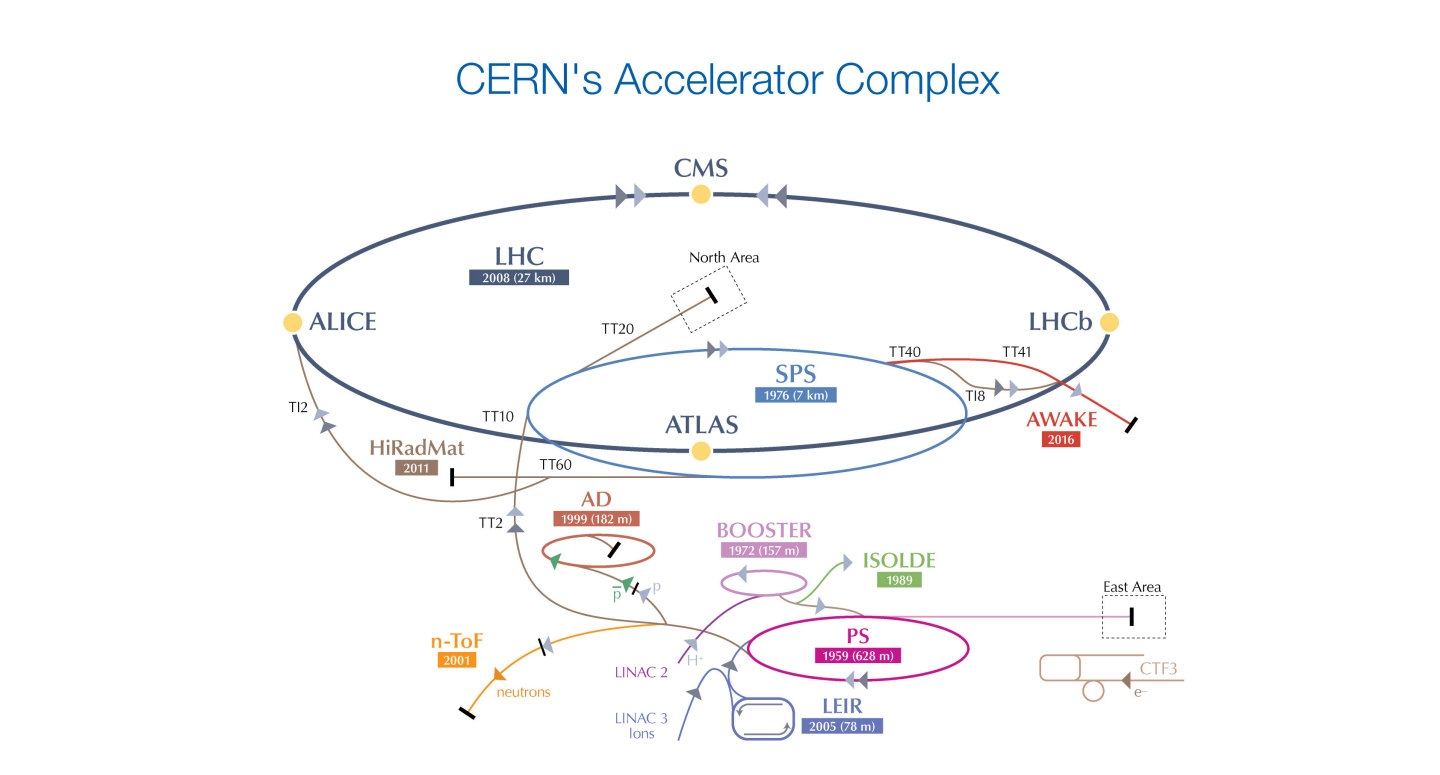
\includegraphics[width=17cm,height=11cm]{Chapter1/cern.jpg}
\caption[Large hadron collider from CERN]{Large hadron collider from CERN\cite{cern1}} \label{lhc}
\end{figure}


Protons in the LHC start out as hydrogen atoms stripped of their electrons. The first accelerating stage the protons are subjected to is a linear accelerator, Linac2,
which accelerates them up to 50 MeV. The protons are then sent into the
Proton Synchotron Booster which accelerates them up to 1.4 GeV before sending them to the Proton Synchotron (PS). The protons leave the PS at 25 GeV before entering the Super Proton Synchotron (SPS), which accelerates them to the LHC injection energy of 450 GeV. After this stage, the beam is ready to be injected into
the LHC through one of two injection lines with 6.5 TeV.\cite{cern3}

\begin{table}[!htbp]
\centering
	\caption[Accelerator operation energies]{Accelerator operation energies\cite{cern3,cern1}}
	\begin{tabular}{|c|c|}
		\hline
		Accelerator & Energy \\
		\hline
		Linac 2 & 50 MeV \\
		\hline
		PS Booster & 1.4 GeV \\
		\hline
		Proton Scyncroton (PS) & 25 GeV\\
		\hline
		SPS & 450 GeV\\
		\hline
		LHC & 6.5 TeV\\
		\hline
	\end{tabular}
\end{table}
\pagebreak
Inside the detectors, collided protons generates an amount of particles such as pion and kaons, which are the most commons, created by the jet particles that were created after the collision. Besides of the particles created by the quarks of the proton, gluons are also radiated and create new particles and photons are radiated too. \\
During the collision time, the main detectors of LHC capture the energy 
and save the data in supercomputers. Those high end computers starts to measure the signals in order to assign a type of events.
\\

The main objective of the LHC is to study the nature of electroweak symmetry breaking for the Higgs mechanism of the SM. 
Alternatives to the Standard Model that involves different symmetries are also put on test. With the exploration of theses theories, people hope for a discovery that guide them toward a unified theory, so the importance to accelerate particles to higher energy scales.
\\
The LHC has a schedule where there is a period of experiments that last for three or four years. Ending the experimental time, the engineers of the LHC start the maintenance.

\begin{figure}[!htbp]
\centering
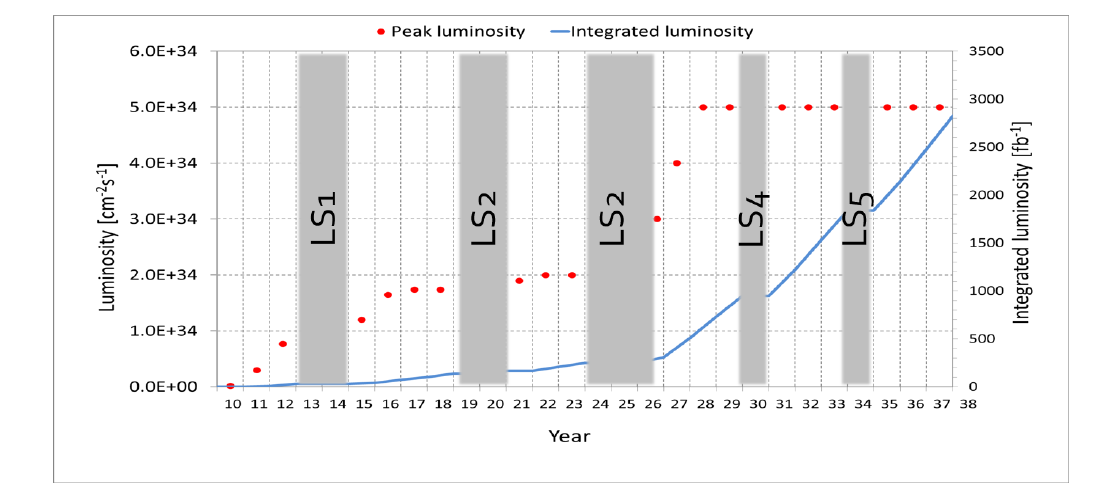
\includegraphics[scale=0.5]{Chapter2/lum6.png}
\caption[LHC schedule, including future plans for increase the center of mass energy and luminosity. The periods labeled LS are the maintenance periods]{LHC schedule, including future plans for increase the center of mass energy and luminosity. The periods labeled LS are the maintenance periods\cite{cern3}.}
\label{lhc-lumi}
\end{figure}
From the figure \ref{lhc-lumi}, shows the Large Hadron Collider forecast for the increase of luminosity for the next years. Red dots are peak luminosity expected to reach and blue line is integrated luminosity. In the year 2018, the maximum integrated luminosity is around 150 $fb^{-1}$\cite{cern3}. From 2019 to 2021 the second phase of maintenance, where engineers increase the performance of the accelerator, give maintenance to the system and introduce new components to the complex. After that period, the LHC starts new collision period at even higher energies in order to explore new particle phenomena.

\pagebreak

\section{The Compact Muon Solenoid}	
The Compact Muon Solenoid (CMS) is a detector with multiple uses in the LHC and part of the main experiments at CERN. Located underground in the France- Switzerland border, in the city of Cessy, France.
This detector was designed in the early 1990s, based on the mass limit of the Higgs boson, and put on operation in 2008, it has a big solenoid that generates a great magnetic field of 4 teslas with the objective to separate particles after a particle collision.
 The detector is 21 meters long, 15 meters wide, 15 meters high, it has a diameter of 5.9 m with a weight of 12000 ton. The reason for such a strong magnetic field is to obtain a better momentum resolution.
 The magnetic flux is returned via a 1.5 m thick iron yoke instrumented with four stations of muon
 chambers.



\begin{figure}[!htbp]
	\centering
	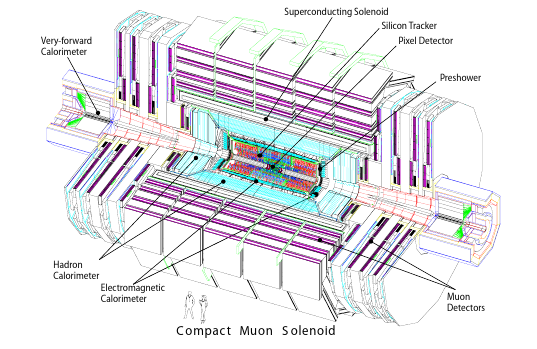
\includegraphics[width=10cm,height=6cm]{Chapter2/cms2.png}
	\caption[View of Compact muon solenoid (CMS)]{View of Compact muon solenoid (CMS)\cite{cms-manual}}\label{cms}
\end{figure}
There are many layers of detectors to register different kinds of energy signals. But since muons go through materials very easy, the complex is buried 100 meters underground.\\ 

The CMS experiment is composed of several detector layers that allow identify and save different types of energy signals and it is saved in a powerful supercomputers that separate and classify the data according to certains variables. The general parts of the CMS are the Silicon Tracker, an Electromagnetic Calorimeter, a Hadron Calorimeter, the solenoid (superconducting magnet) and the Muon Detector. \\

\begin{table}[ht]
	\caption[Characteristic of the CMS superconducting solenoid]{Characteristic of the CMS superconducting solenoid\cite{cms-manual}}
	\centering
	\begin{tabular}{|c|c|}
		\hline
		Field strength & 4 T \\
		Inner Bore & 5.9 m \\
		Length & 12.9 m\\
		Number of Turns & 2168\\
		Current & 19.5 kA\\
		Stored energy & 2.7 GJ\\
		\hline
	\end{tabular}
	\label{tab:my_label}
\end{table}



%The trigger or event selection process must reduce the approximately 1 billion interactions per second to more less than 100 events per second for storage and subsequent analysis.\\

 The objectives of the CMS experiment are numerous. One of them is
identification of muons by measuring the momenta and scattering angle. Muons can be produced in interesting events like Higgs, $W^{\pm}$ and $Z$ boson decays.%Search for evidence and give proof of super symmetry for show evidence of BSM (Beyond Standard Model). Detection of massive vector bosons $W^\pm$ and Z via $e^+e^-$ and $\mu^+ \mu^-$ decays.\\
%Search for extra dimensions from BSM theory that could be related to production of particles and quantum gravity. Study of QCD, electroweak and flavor physics to detect new decays predicted by SM at higher energies. Heavy ions collision experiments for the study of production of very strongly interacting nuclear matter\cite{cms-manual}.
This experiment along the ATLAS experiment discovered the Higgs boson in 2012.
\\


\subsection{Silicon Tracker}
The Silicon Tracker is the first of the main subdetectors of CMS from inside to outside. The Tracker is composed of two sub components: Pixel and Strip detectors. The outer radius of the tracker is 110 cm, and its total length is 540 cm. The tracker coverage is $|\eta|<2.4$\footnote{$\eta$, called pseudorapidity, is a coordinate where $\eta=-\ln{\tan{\frac{\theta}{2}}}$}.\\

In the Pixel barrel section, there are 3 layers of pixel sensors with radii of 4.4, 7.3 and 10.2 cm with a length of 53 cm. Each pixel has an area of 100 $\times$ 150 $\mu m^2$. The barrel section has 768 pixel modules.
%The barrel section of the silicon tracker is divided in inner and outer barrel, where the inner section is shorter than outer barrel along with 3 inner disk between the transition region between barrel and endcap sections because avoids shallow track crossing angles. 
The Pixel endcap has 2 disks on each side placed at 34.6 and 46.5 cm in the z axis. Each disk covers radii from 6 to 15 cm and is divided into 24 blades with 7 modules each blade.
They are assembled in a turbine-like geometry that contains a total of 672 pixel modules. %with 7
%different modules in each blade.
\\

 %The outer radius of the tracker is 110 cm, and its total length is 540 cm. \\
 %Here, silicon microstrip detectors are placed in the r axis (cylindrical coordinates), between 20 and 110 cm.
%In the endcap section 2 pixel and microstrip layers are placed in each endcap. The endcap have 2 disks of radii from 6 to 15 cm placed at 34.6 and 46.5 cm in the z axis. The endcap disks comprise 672 pixel modules with 7
%different modules in each blade.
The Strip Detector is divided in 4 sections: Tracker inner barrel (TIB), tracker outer barrel (TOB), tracker encap (TEC) and tracker inner disk (TID). The region that cover the barrel section is $|z|<65$ cm for TIB and $|z|<110$cm for TOB. The first two are composed of silicon sensors layers of 4 and 6 layers respectively. The TEC has 9 disk extending in the region 120 cm > $|z|$ > 280 cm. The 
TID comprises 3 small disks that fill the gap between the TIB and the TEC.


The Strip Detector have almost 15 400 modules, mounted on
carbon-fiber structures and housed inside by a temperature controlled outer support tube. The operating temperature must be around -$\ang{20}$C. 
The total area of the pixel detector is around 1 $m^2$ and the silicon strips is 200 m$^2$. 
The inner tracker comprises 66 million pixels and 9.6
million silicon strips \cite{cms-manual}.
A full coverage of the Tracker is shown in figure \ref{pixel2}
\\

\begin{figure}[ht]
	\centering
	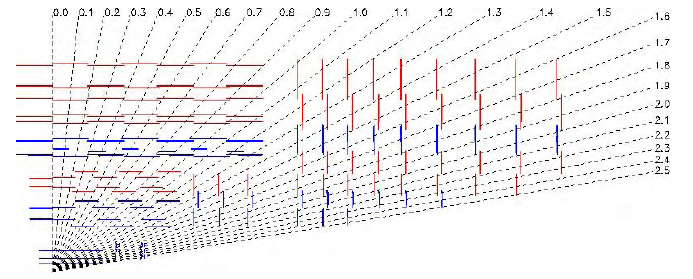
\includegraphics[scale=0.7]{Chapter2/pixel2.png}
	\caption[The Tracker layout distributed in terms of $\eta$]{The Tracker layout distributed in terms of $\eta$\cite{cms-manual}.}
	\label{pixel2}
\end{figure}
During the particle collision, it generates a lot of different particles that pass first through the inner tracker, interacting with the sensors layers and registering the particle path.
By reconstructing the path of the particles, it is possible to generate a track, which allows to measure the momentum of the particle by calculating its curvature. The tracker is used to reconstruct the path of charged particles (e.g. electrons, muons, pions). The most important objects of study are the momentum and the vertex (origin of the track). The efficiency of the tracker is estimated by using samples of muons and pions with $p_t$ of 1,10 and 100 GeV. 
For muons the efficiency of the tracker is shown in \ref{efi}
\begin{figure}[!htbp]
	\centering
	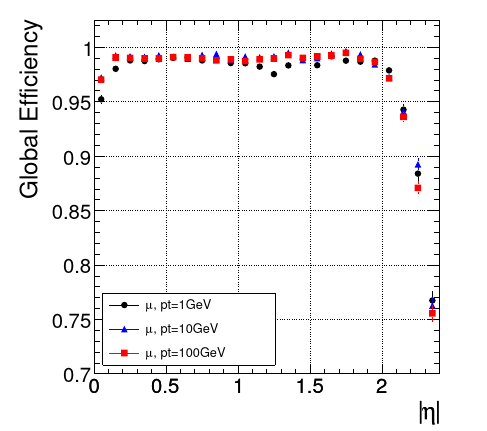
\includegraphics[width=10cm,height=6cm]{Chapter2/tracker.png}
	\caption[Total reconstruction efficiency for muons]{Total reconstruction efficiency for muons\cite{cms-manual} }\label{efi}
\end{figure}
\\
According to figure \ref{efi}, the efficiency of the tracker is around 98 $\%$ for $|\eta|<2$. The resolution of the tracker for muons with $p_t$=100 GeV is around 1-2 $\%$.\\
Of course, this is a first stage of the measurement of particle momentum because the other detectors are used to increase and improve the measurement and reconstruction of the particle path.

\subsection{Electromagnetic calorimeter}

The electromagnetic calorimeter or ECAL is a calorimeter composed of 61200 lead tungstate (PbWO$_4$) crystals that act as scintillating crystals (emits light when particles interact with the crystal). These calorimeters are mounted in the central barrel and closed by 7324 crystals in the both endcaps. The barrel section of the ECAL covers the range $|\eta| < 1.479$. The crystals in the barrel have a pyramid shape and their cross section is 22$\times$22 mm$^2$ at the front face and 26$\times$26 mm$^2$ at rear face. The crystal length is 230 mm. The EB (barrel section of ECAL) has a inner radius of 129 cm\cite{cms-manual}\\

The endcaps cover have the range 1.479 < $|\eta|$ < 3.0. The distance between the interaction point and the endcap is 3.144 m. The endcap has identically shaped crystals grouped in
mechanical units of 5×5 crystals. The crystal cross section for the rear face is 30 $\times$ 30 mm$^2$, and for front face cross section is 28.62 $\times$ 28.62 mm$^2$ with length of 220 mm.
\\
\begin{figure}[!htbp]
	\centering
	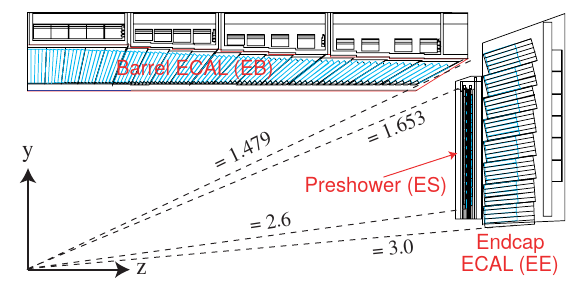
\includegraphics[width=10cm,height=6cm]{Chapter2/ecal.png}
	\caption[View of the ECAL]{View of the ECAL\cite{cms-manual}}\label{ecal}
\end{figure}
In the barrel, there are photo detectors called avalanche photo diodes (APD), made of silicon with a active area of 5 $\times$ 5 mm$^2$ with 2 glued to the back of each crystal. At the endcap, the photo detectors are vacuum photo diodes (VPT), made of with an anode of copper mesh (10 $\mu m$), allowing to operate in the magnetic field. VPT have a size of 25 mm in diameter, glued to the back of each crystal.\\


There is also a preshower detector, which principal function is to identify neutral pions in the
endcaps within the region 1.653 < |$\eta$| < 2.6. It also helps the identification of electrons
against minimum ionizing particles, and improves the position determination of electrons and photons.
\\

As its name says, the ECAL is mainly used for the electron detection, but also detects, photons, and neutral pions. The charged particles reach the crystals that provokes the photo diodes detect energy.\\
The resolution of the ECAL is estimated by using a test beam and registering the energy signals. The resolution for electrons with energies of 120 GeV, it has obtained a resolution of 0.5$\%$.
 
 %that a electron is separated, and regrouping in other place due to the electric field generated by the voltage source. 
 %The ES is a sampling calorimeter with 2 layers: lead
%radiators initiate electromagnetic showers from incoming photons/electrons whilst silicon
%strip sensors placed after each radiator measure the energy deposited and the transverse shower profiles.


\subsection{Hadron calorimeter}
The hadron calorimeter (HCAL) along the ECAL, form a complete calorimeter that allows to measure the jets and missing transverse energy. HCAL is located in the barrel and the endcaps, surrounding the ECAL and affected by the magnetic field generated by the solenoid. The Barrel section (HB) and endcap section (HE) cover the pseudorapidity 0 < $|\eta|$ < 1.3 and 1.3 < $|\eta|$ < 3.0 respectively.\\ 


The HB is an assembly of two half barrels, composed of 18 wedges. Each wedge has 17 active layers composed of scintillator tiles with 16 layers of absorber metal (brass and stainless steel). Each tile has a size of $\Delta \eta × \Delta \phi$ = 0.087 $\times$ 0.087. Light of scintillator is collected by a single wave
length shifting fiber (WLS) for each scintillator tile. The wedge has a inner radius of 1777 mm to an outer radius of 2876.5 mm. 
\\

HE is composed by brass absorber plates, with the thickness of 78 mm, and a total of 19 scintillator layers with a thickness of 3.7 mm. HE is sectioned in 5 in $\phi$ to match the barrel wedges.
. %HO scintillators follow the HCAL barrel tower geometry in $\eta$ and angle $\phi$, that is, the geometry of the barrel muon system. Divided by 5 rings of 2.54 wide, composed of the scintillators on either side of the tail catcher iron of 18cm thick at radial distances of 3850 and 4097 mm respectively. \cite{cms-manual} 
\\
\begin{figure}[!htbp]
	\centering
	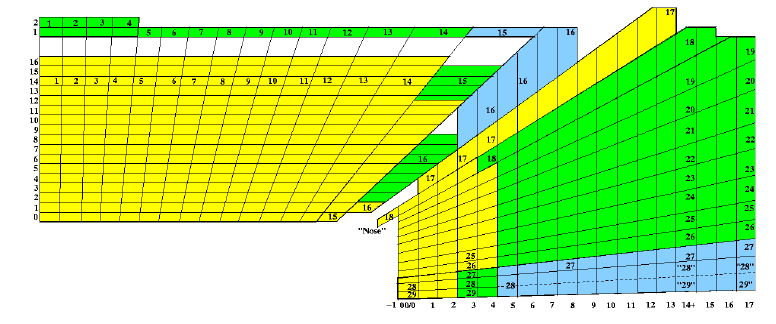
\includegraphics[width=10cm,height=6cm]{Chapter2/hcal.png}
	\caption[View of the CMS HCAL showing the different layers and tower regions. In the endcap, the towers are defined with two longitudinal segments as shown by the colors]{View of the CMS HCAL showing the different layers and tower regions. In the endcap, the towers are defined with two longitudinal segments as shown by the colors\cite{cms-manual}}\label{hcal}
\end{figure}
The outer barrel hadron calorimeter (HO) consists of layers of scintillator with thickness of 10 mm, located outside of the
magnet coil that cover the region -1.26 < $|\eta|$ < 1.26.\\
There is also a foward calorimeter (HF) located at 11.2 m from the interaction point, that cover the region of 2.9 < $|\eta|$ < 5. They are made of
steel absorber and embedded radiation hard quartz fibers, which collects 
Cherenkov light\cite{cms-manual}.% that is when a charged particle travels through matter faster than light can, resulting in a blue light emmision of the material. 
%The length of the fibers are 1.65 m and 1.43 m, which are alterned with a 5 mm of separation. 
\\
 
The tiles are arranged in a tower pattern in the $\eta-\phi$ space, projective to the interaction point. In total there
are 4176 towers. The towers are used as input to several jet reconstruction algorithms.

The HCAL measures the energy of hadrons, such as the pions and kaons. 
The energy resolution of the HCAL was estimated using a test beam of pions. For 100 GeV pions, the resolution obtained is 12$\%$.
 %By using the info given by the HCAL, it is possible reconstruct the track in order to calculate the momentum of the particles. 

\subsection{Muon Detector}
%The muon detector system %has 3 primary functions: muon
%triggering, identification, and momentum measurement\cite{cms7}. 
%The process utilized in the CMS muon chamber systems is gas ionization. Those gas-ionization particle detectors are arranged in a cylindrical barrel region and planar endcaps, in order to meet the geometry of the solenoid. The barrel detector is built with 4 layers of 250 chambers inside the magnet return yoke.\cite{cms-manual}
The Muon Detector has three main subdetectors: the drift tubes chambers (DT), the cathode strips chambers (CSC) and the resistive plate chamber (RPC). 
The DT's, CSC's and RPC's are shown in the figure \ref{dt}.
 \\
 
The DT chambers cover the barrel section $|\eta|<1.2$, composed of rectangular gas filled active cells. Those cells have a transverse size of 42 $\times$ 13 mm$^2$ with a 50 $\mu m$ diameter anode wire at the center that operates at voltages of over 3600 V. The gas used in this cells is a mix of Ar and CO$_2$ with a proportion of 85 $\%$ and 15 $\%$. There are 250 chambers in 4 layers inside the magnet return yoke, with radii of approximately 4.0, 4.9, 5.9 and 7.0 m from the beam axis and 12 sections covering 30$^\circ$ in $\phi$ each one.
\\
\begin{figure}[!htbp]
	\centering
	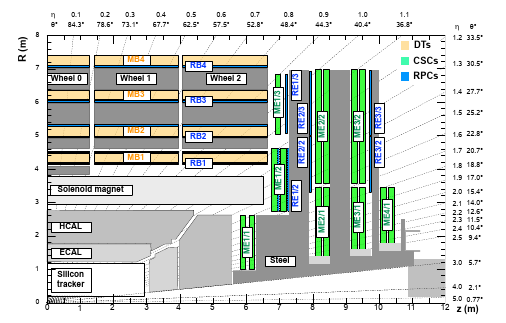
\includegraphics[width=11cm,height=7cm]{Chapter2/csc}
	\caption[Cross section of a quadrant of the CMS with axis parallel to the beam (z axis) horizontally and the radius of the detector in terms of the $\eta$]{Cross section of a quadrant of the CMS with axis parallel to the beam (z axis) horizontally and the radius of the detector in terms of the $\eta$\cite{cms-manual}.}
	\label{dt}
\end{figure}

The CSC's are located in the endcap regions 0.9 < $|\eta|$ < 2.4. The CSC's are installed on the face of steel disks perpendicular to the beam. 
Each CSC has a trapezoidal shape and consist of 6 gas gaps between 7 metal plates, where each gap contains copper cathode strips and anode wires running almost perpendicularly to
the strips, with a diameter of 50 $\mu m$ separated by 3.16 mm. 
%CSC is composed of 6 layers that measures the $\mu$ position in the r-$\phi$ coordinate plane. 
The chambers use a gas mixture of 50$\%$ CO$_2$, 40 $\%$ Ar and 10$\%$ CF$_4$. The muon endcap system comprises 468 CSCs in the 2 endcaps \cite{cms-manual,cms7}.
%Together with DT, cover the $|\eta|< 2.4$. These systems can each identify the collision crossing that generated the muon and trigger on (recolect) the transverse momentum ($p_T$). 
\\

The RPC are located in the barrel and endcap regions that covers the range o $|\eta|<1.6$. The main purpose is to trigger events with muons. 
RPC's are structured with a double gas filled gap and readout strips between the gaps.\\
 The gas mix used in the RPC consist of 95.2$\%$ Freon
($C_2 H_2 F_4$ ), 4.5$\%$ isobutane ($C_4 H_{10}$), and 0.3$\%$ sulphur hexafluoride (SF$_6$ )\cite{cms7}.\\


 %The vertical lines represent the endcap and the horizontal the muon barrel. The orange sections are the DTs, where the 4 DTs are labeled MB,CSC marked in green are labeled ME or muon endcap and RPC are the blue lines that are located in the barrel and the endcap. RPC are labeled RB and RE respectively. 

%The produced muons are measured in three zones: in the inner tracker, after the coil, and in
%the return flux. Measurement the momentum of muons in the muon detector is determined by the muon bending angle at the exit of the 4T coil with the interaction point as the origin of the muon\cite{cms7}\cite{cms-manual}.
%The resolution of the muom detector is based on simulations taking account with the geometry and a test beam. 
The main purpose of the Muon System Detector is to identify muon tracks. 
The efficiency of the muon system is estimated by using single muon samples simulated with $p_t$=10, 50, 100, 500 and 1000 GeV. The results are shown in the figure \ref{mu-efi}.
\begin{figure}
	\centering
	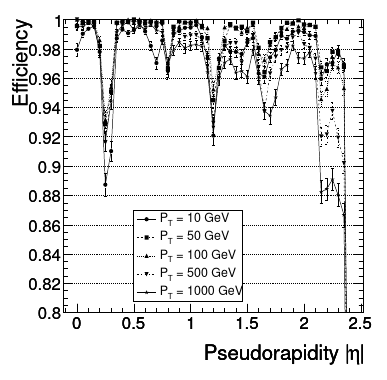
\includegraphics[width=0.4\linewidth]{Chapter2/mu-efi}
	\caption[Muon reconstruction efficiency in terms of $\eta$ and $p_t$]{Muon reconstruction efficiency in terms of $\eta$ and $p_t$\cite{cms-manual}}
	\label{mu-efi}
\end{figure}
The graph shows an efficiency of approximately 98$\%$ in the the fully instrumented regions. In the intersection regions, there are drops in efficiency due to the separation of the chambers. % There is a reduction of the efficiency to 6$\%$, which corresponds to the $\eta$ position for the separation.
